%%===========================================================%%
%%                                                           %%
%%              ENERGY LOSS CORRECTION APPENDIX            	%%
%%                                                           %%
%%===========================================================%%

\chapter{Energy Loss Correction}\label{appendix:energyLoss}
\begin{figure}[H]
\caption[Energy loss correction for $\pi^-$ as a function of reconstructed transverse momentum $p_T^{meas}$.]{Energy loss correction $p_T^{meas}-p_T^{true}$ for $\pi^-$ as a function of reconstructed transverse momentum $p_T^{meas}$ $\left(|\eta|<0.7\right)$ in single $z$-vertex bin whose range is given on each plot. Red lines and arrows indicate region accepted in analyses. One can notice an offset of about $3-4$~MeV for negative $z$-vertex. It is a known issue with STAR simulation where HFT support material is badly described for negative $z<-30$~cm.}\label{fig:energyLossPrimaryPi_minus}
\centering
\parbox{0.329\textwidth}{
  \centering
  \includegraphics[width=\linewidth,page=3]{graphics/energyLoss/energyLoss3D_OnePrtAlso.pdf}\\
  \includegraphics[width=\linewidth,page=6]{graphics/energyLoss/energyLoss3D_OnePrtAlso.pdf}\\
  \includegraphics[width=\linewidth,page=9]{graphics/energyLoss/energyLoss3D_OnePrtAlso.pdf}\\
  \includegraphics[width=\linewidth,page=12]{graphics/energyLoss/energyLoss3D_OnePrtAlso.pdf}\\
  \includegraphics[width=\linewidth,page=15]{graphics/energyLoss/energyLoss3D_OnePrtAlso.pdf}\\
}~
\parbox{0.329\textwidth}{
  \centering
  \includegraphics[width=\linewidth,page=4]{graphics/energyLoss/energyLoss3D_OnePrtAlso.pdf}\\
  \includegraphics[width=\linewidth,page=7]{graphics/energyLoss/energyLoss3D_OnePrtAlso.pdf}\\
  \includegraphics[width=\linewidth,page=10]{graphics/energyLoss/energyLoss3D_OnePrtAlso.pdf}\\
  \includegraphics[width=\linewidth,page=13]{graphics/energyLoss/energyLoss3D_OnePrtAlso.pdf}\\
  \includegraphics[width=\linewidth,page=16]{graphics/energyLoss/energyLoss3D_OnePrtAlso.pdf}\\
}%
\parbox{0.329\textwidth}{
  \centering
  \includegraphics[width=\linewidth,page=5]{graphics/energyLoss/energyLoss3D_OnePrtAlso.pdf}\\
  \includegraphics[width=\linewidth,page=8]{graphics/energyLoss/energyLoss3D_OnePrtAlso.pdf}\\
  \includegraphics[width=\linewidth,page=11]{graphics/energyLoss/energyLoss3D_OnePrtAlso.pdf}\\
  \includegraphics[width=\linewidth,page=14]{graphics/energyLoss/energyLoss3D_OnePrtAlso.pdf}\\
  \includegraphics[width=\linewidth,page=17]{graphics/energyLoss/energyLoss3D_OnePrtAlso.pdf}\\
}%
\end{figure}
\vspace{-3.5em}
\begin{figure}[H]\ContinuedFloat
% ~\\[32pt]
\parbox{0.329\textwidth}{
  \includegraphics[width=\linewidth,page=18]{graphics/energyLoss/energyLoss3D_OnePrtAlso.pdf}\\
}~
\end{figure}
%%%pi+
\begin{figure}[H]
\caption[Energy loss correction for $\pi^+$ as a function of reconstructed transverse momentum $p_T^{meas}$.]{Energy loss correction $p_T^{meas}-p_T^{true}$ for $\pi^+$ as a function of reconstructed transverse momentum $p_T^{meas}$ $\left(|\eta|<0.7\right)$ in single $z$-vertex bin whose range is given on each plot. Red lines and arrows indicate region accepted in analyses. One can notice an offset of about $3-4$~MeV for negative $z$-vertex. It is a known issue with STAR simulation where HFT support material is badly described for negative $z<-30$~cm.}\label{fig:energyLossPrimaryPi_plus}
\parbox{0.329\textwidth}{
  \includegraphics[width=\linewidth,page=63]{graphics/energyLoss/energyLoss3D_OnePrtAlso.pdf}\\
  \includegraphics[width=\linewidth,page=66]{graphics/energyLoss/energyLoss3D_OnePrtAlso.pdf}\\
  \includegraphics[width=\linewidth,page=69]{graphics/energyLoss/energyLoss3D_OnePrtAlso.pdf}\\
  \includegraphics[width=\linewidth,page=72]{graphics/energyLoss/energyLoss3D_OnePrtAlso.pdf}\\
  \includegraphics[width=\linewidth,page=75]{graphics/energyLoss/energyLoss3D_OnePrtAlso.pdf}\\
}~
\parbox{0.329\textwidth}{
  \includegraphics[width=\linewidth,page=64]{graphics/energyLoss/energyLoss3D_OnePrtAlso.pdf}\\
  \includegraphics[width=\linewidth,page=67]{graphics/energyLoss/energyLoss3D_OnePrtAlso.pdf}\\
  \includegraphics[width=\linewidth,page=70]{graphics/energyLoss/energyLoss3D_OnePrtAlso.pdf}\\
  \includegraphics[width=\linewidth,page=73]{graphics/energyLoss/energyLoss3D_OnePrtAlso.pdf}\\
  \includegraphics[width=\linewidth,page=76]{graphics/energyLoss/energyLoss3D_OnePrtAlso.pdf}\\
}%
\parbox{0.329\textwidth}{
  \includegraphics[width=\linewidth,page=65]{graphics/energyLoss/energyLoss3D_OnePrtAlso.pdf}\\
  \includegraphics[width=\linewidth,page=68]{graphics/energyLoss/energyLoss3D_OnePrtAlso.pdf}\\
  \includegraphics[width=\linewidth,page=71]{graphics/energyLoss/energyLoss3D_OnePrtAlso.pdf}\\
  \includegraphics[width=\linewidth,page=74]{graphics/energyLoss/energyLoss3D_OnePrtAlso.pdf}\\
  \includegraphics[width=\linewidth,page=77]{graphics/energyLoss/energyLoss3D_OnePrtAlso.pdf}\\
}%
\end{figure}

\begin{figure}[H]\ContinuedFloat
% ~\\[32pt]
\vspace{-3.5em}
\parbox{0.329\textwidth}{
  \includegraphics[width=\linewidth,page=78]{graphics/energyLoss/energyLoss3D_OnePrtAlso.pdf}\\
  \vspace{-4em}
}~
\end{figure}
%%%K+
\begin{figure}[H]
\caption[Energy loss correction for $K^+$ as a function of reconstructed transverse momentum $p_T^{meas}$.]{Energy loss correction $p_T^{meas}-p_T^{true}$ for $K^+$ as a function of reconstructed transverse momentum $p_T^{meas}$ $\left(|\eta|<0.7\right)$ in single $z$-vertex bin whose range is given on each plot. Red lines and arrows indicate region accepted in analyses.}\label{fig:energyLossPrimaryK_plus}
\parbox{0.329\textwidth}{
  \includegraphics[width=\linewidth,page=83]{graphics/energyLoss/energyLoss3D_OnePrtAlso.pdf}\\
  \includegraphics[width=\linewidth,page=86]{graphics/energyLoss/energyLoss3D_OnePrtAlso.pdf}\\
  \includegraphics[width=\linewidth,page=89]{graphics/energyLoss/energyLoss3D_OnePrtAlso.pdf}\\
  \includegraphics[width=\linewidth,page=92]{graphics/energyLoss/energyLoss3D_OnePrtAlso.pdf}\\
  \includegraphics[width=\linewidth,page=95]{graphics/energyLoss/energyLoss3D_OnePrtAlso.pdf}\\
}~
\parbox{0.329\textwidth}{
  \includegraphics[width=\linewidth,page=84]{graphics/energyLoss/energyLoss3D_OnePrtAlso.pdf}\\
  \includegraphics[width=\linewidth,page=87]{graphics/energyLoss/energyLoss3D_OnePrtAlso.pdf}\\
  \includegraphics[width=\linewidth,page=90]{graphics/energyLoss/energyLoss3D_OnePrtAlso.pdf}\\
  \includegraphics[width=\linewidth,page=93]{graphics/energyLoss/energyLoss3D_OnePrtAlso.pdf}\\
  \includegraphics[width=\linewidth,page=96]{graphics/energyLoss/energyLoss3D_OnePrtAlso.pdf}\\
}%
\parbox{0.329\textwidth}{
  \includegraphics[width=\linewidth,page=85]{graphics/energyLoss/energyLoss3D_OnePrtAlso.pdf}\\
  \includegraphics[width=\linewidth,page=88]{graphics/energyLoss/energyLoss3D_OnePrtAlso.pdf}\\
  \includegraphics[width=\linewidth,page=91]{graphics/energyLoss/energyLoss3D_OnePrtAlso.pdf}\\
  \includegraphics[width=\linewidth,page=94]{graphics/energyLoss/energyLoss3D_OnePrtAlso.pdf}\\
  \includegraphics[width=\linewidth,page=97]{graphics/energyLoss/energyLoss3D_OnePrtAlso.pdf}\\
}%
\end{figure}

\begin{figure}[H]\ContinuedFloat
% ~\\[32pt]
\vspace{-3.5em}
\parbox{0.329\textwidth}{
  \includegraphics[width=\linewidth,page=98]{graphics/energyLoss/energyLoss3D_OnePrtAlso.pdf}\\
  \vspace{-4em}
}~
\end{figure}
%%%pbar
\begin{figure}[H]
\caption[Energy loss correction for $\bar{p}$ as a function of reconstructed transverse momentum $p_T^{meas}$.]{Energy loss correction $p_T^{meas}-p_T^{true}$ for $\bar{p}$ as a function of reconstructed transverse momentum $p_T^{meas}$ $\left(|\eta|<0.7\right)$ in single $z$-vertex bin whose range is given on each plot. Red lines and arrows indicate region accepted in analyses.}\label{fig:energyLossPrimaryP_bar}
\parbox{0.329\textwidth}{
  \includegraphics[width=\linewidth,page=43]{graphics/energyLoss/energyLoss3D_OnePrtAlso.pdf}\\
  \includegraphics[width=\linewidth,page=46]{graphics/energyLoss/energyLoss3D_OnePrtAlso.pdf}\\
  \includegraphics[width=\linewidth,page=49]{graphics/energyLoss/energyLoss3D_OnePrtAlso.pdf}\\
  \includegraphics[width=\linewidth,page=52]{graphics/energyLoss/energyLoss3D_OnePrtAlso.pdf}\\
  \includegraphics[width=\linewidth,page=55]{graphics/energyLoss/energyLoss3D_OnePrtAlso.pdf}\\
}~
\parbox{0.329\textwidth}{
  \includegraphics[width=\linewidth,page=44]{graphics/energyLoss/energyLoss3D_OnePrtAlso.pdf}\\
  \includegraphics[width=\linewidth,page=47]{graphics/energyLoss/energyLoss3D_OnePrtAlso.pdf}\\
  \includegraphics[width=\linewidth,page=50]{graphics/energyLoss/energyLoss3D_OnePrtAlso.pdf}\\
  \includegraphics[width=\linewidth,page=53]{graphics/energyLoss/energyLoss3D_OnePrtAlso.pdf}\\
  \includegraphics[width=\linewidth,page=56]{graphics/energyLoss/energyLoss3D_OnePrtAlso.pdf}\\
}%
\parbox{0.329\textwidth}{
  \includegraphics[width=\linewidth,page=45]{graphics/energyLoss/energyLoss3D_OnePrtAlso.pdf}\\
  \includegraphics[width=\linewidth,page=48]{graphics/energyLoss/energyLoss3D_OnePrtAlso.pdf}\\
  \includegraphics[width=\linewidth,page=51]{graphics/energyLoss/energyLoss3D_OnePrtAlso.pdf}\\
  \includegraphics[width=\linewidth,page=54]{graphics/energyLoss/energyLoss3D_OnePrtAlso.pdf}\\
  \includegraphics[width=\linewidth,page=57]{graphics/energyLoss/energyLoss3D_OnePrtAlso.pdf}\\
}%
\end{figure}

\begin{figure}[H]\ContinuedFloat
% ~\\[32pt]
\vspace{-3.5em}
\parbox{0.329\textwidth}{
  \includegraphics[width=\linewidth,page=58]{graphics/energyLoss/energyLoss3D_OnePrtAlso.pdf}\\
  \vspace{-4em}
}~
\end{figure}
%%%p
\begin{figure}[H]
\caption[Energy loss correction for $p$ as a function of reconstructed transverse momentum $p_T^{meas}$.]{Energy loss correction $p_T^{meas}-p_T^{true}$ for $p$ as a function of reconstructed transverse momentum $p_T^{meas}$ $\left(|\eta|<0.7\right)$ in single $z$-vertex bin whose range is given on each plot. Red lines and arrows indicate region accepted in analyses.}\label{fig:energyLossPrimaryP}
\parbox{0.329\textwidth}{
  \includegraphics[width=\linewidth,page=103]{graphics/energyLoss/energyLoss3D_OnePrtAlso.pdf}\\
  \includegraphics[width=\linewidth,page=106]{graphics/energyLoss/energyLoss3D_OnePrtAlso.pdf}\\
  \includegraphics[width=\linewidth,page=109]{graphics/energyLoss/energyLoss3D_OnePrtAlso.pdf}\\
  \includegraphics[width=\linewidth,page=112]{graphics/energyLoss/energyLoss3D_OnePrtAlso.pdf}\\
  \includegraphics[width=\linewidth,page=115]{graphics/energyLoss/energyLoss3D_OnePrtAlso.pdf}\\
}~
\parbox{0.329\textwidth}{
  \includegraphics[width=\linewidth,page=104]{graphics/energyLoss/energyLoss3D_OnePrtAlso.pdf}\\
  \includegraphics[width=\linewidth,page=107]{graphics/energyLoss/energyLoss3D_OnePrtAlso.pdf}\\
  \includegraphics[width=\linewidth,page=110]{graphics/energyLoss/energyLoss3D_OnePrtAlso.pdf}\\
  \includegraphics[width=\linewidth,page=113]{graphics/energyLoss/energyLoss3D_OnePrtAlso.pdf}\\
  \includegraphics[width=\linewidth,page=116]{graphics/energyLoss/energyLoss3D_OnePrtAlso.pdf}\\
}%
\parbox{0.329\textwidth}{
  \includegraphics[width=\linewidth,page=105]{graphics/energyLoss/energyLoss3D_OnePrtAlso.pdf}\\
  \includegraphics[width=\linewidth,page=108]{graphics/energyLoss/energyLoss3D_OnePrtAlso.pdf}\\
  \includegraphics[width=\linewidth,page=111]{graphics/energyLoss/energyLoss3D_OnePrtAlso.pdf}\\
  \includegraphics[width=\linewidth,page=114]{graphics/energyLoss/energyLoss3D_OnePrtAlso.pdf}\\
  \includegraphics[width=\linewidth,page=117]{graphics/energyLoss/energyLoss3D_OnePrtAlso.pdf}\\
}%
\end{figure}

\begin{figure}[H]\ContinuedFloat
% ~\\[32pt]
\vspace{-3.5em}
\parbox{0.329\textwidth}{
  \includegraphics[width=\linewidth,page=118]{graphics/energyLoss/energyLoss3D_OnePrtAlso.pdf}\\
  \vspace{-4em}
}~
\end{figure}
%%%negative
\begin{figure}[H]
\caption[Energy loss correction for negative particles as a function of reconstructed transverse momentum $p_T^{meas}$.]{Energy loss correction $p_T^{meas}-p_T^{true}$ for negative particles as a function of reconstructed transverse momentum $p_T^{meas}$ $\left(|\eta|<0.7\right)$ in single $z$-vertex bin whose range is given on each plot. Red lines and arrows indicate region accepted in analyses.}\label{fig:energyLossPrimaryNegative}
\parbox{0.329\textwidth}{
  \includegraphics[width=\linewidth,page=123]{graphics/energyLoss/energyLoss3D_OnePrtAlso.pdf}\\
  \includegraphics[width=\linewidth,page=126]{graphics/energyLoss/energyLoss3D_OnePrtAlso.pdf}\\
  \includegraphics[width=\linewidth,page=129]{graphics/energyLoss/energyLoss3D_OnePrtAlso.pdf}\\
  \includegraphics[width=\linewidth,page=132]{graphics/energyLoss/energyLoss3D_OnePrtAlso.pdf}\\
  \includegraphics[width=\linewidth,page=135]{graphics/energyLoss/energyLoss3D_OnePrtAlso.pdf}\\
}~
\parbox{0.329\textwidth}{
  \includegraphics[width=\linewidth,page=124]{graphics/energyLoss/energyLoss3D_OnePrtAlso.pdf}\\
  \includegraphics[width=\linewidth,page=127]{graphics/energyLoss/energyLoss3D_OnePrtAlso.pdf}\\
  \includegraphics[width=\linewidth,page=130]{graphics/energyLoss/energyLoss3D_OnePrtAlso.pdf}\\
  \includegraphics[width=\linewidth,page=133]{graphics/energyLoss/energyLoss3D_OnePrtAlso.pdf}\\
  \includegraphics[width=\linewidth,page=136]{graphics/energyLoss/energyLoss3D_OnePrtAlso.pdf}\\
}%
\parbox{0.329\textwidth}{
  \includegraphics[width=\linewidth,page=125]{graphics/energyLoss/energyLoss3D_OnePrtAlso.pdf}\\
  \includegraphics[width=\linewidth,page=128]{graphics/energyLoss/energyLoss3D_OnePrtAlso.pdf}\\
  \includegraphics[width=\linewidth,page=131]{graphics/energyLoss/energyLoss3D_OnePrtAlso.pdf}\\
  \includegraphics[width=\linewidth,page=134]{graphics/energyLoss/energyLoss3D_OnePrtAlso.pdf}\\
  \includegraphics[width=\linewidth,page=137]{graphics/energyLoss/energyLoss3D_OnePrtAlso.pdf}\\
}%
\end{figure}

\begin{figure}[H]\ContinuedFloat
% ~\\[32pt]
\vspace{-3.5em}
\parbox{0.329\textwidth}{
  \includegraphics[width=\linewidth,page=138]{graphics/energyLoss/energyLoss3D_OnePrtAlso.pdf}\\
  \vspace{-4em}
}~
\end{figure}
%%%positive
\begin{figure}[H]
\caption[Energy loss correction for positive particles as a function of reconstructed transverse momentum $p_T^{meas}$.]{Energy loss correction $p_T^{meas}-p_T^{true}$ for positive particles as a function of reconstructed transverse momentum $p_T^{meas}$ $\left(|\eta|<0.7\right)$ in single $z$-vertex bin whose range is given on each plot. Red lines and arrows indicate region accepted in analyses.}\label{fig:energyLossPrimaryPositive}
\parbox{0.329\textwidth}{
  \includegraphics[width=\linewidth,page=143]{graphics/energyLoss/energyLoss3D_OnePrtAlso.pdf}\\
  \includegraphics[width=\linewidth,page=146]{graphics/energyLoss/energyLoss3D_OnePrtAlso.pdf}\\
  \includegraphics[width=\linewidth,page=149]{graphics/energyLoss/energyLoss3D_OnePrtAlso.pdf}\\
  \includegraphics[width=\linewidth,page=152]{graphics/energyLoss/energyLoss3D_OnePrtAlso.pdf}\\
  \includegraphics[width=\linewidth,page=155]{graphics/energyLoss/energyLoss3D_OnePrtAlso.pdf}\\
}~
\parbox{0.329\textwidth}{
  \includegraphics[width=\linewidth,page=144]{graphics/energyLoss/energyLoss3D_OnePrtAlso.pdf}\\
  \includegraphics[width=\linewidth,page=147]{graphics/energyLoss/energyLoss3D_OnePrtAlso.pdf}\\
  \includegraphics[width=\linewidth,page=150]{graphics/energyLoss/energyLoss3D_OnePrtAlso.pdf}\\
  \includegraphics[width=\linewidth,page=153]{graphics/energyLoss/energyLoss3D_OnePrtAlso.pdf}\\
  \includegraphics[width=\linewidth,page=156]{graphics/energyLoss/energyLoss3D_OnePrtAlso.pdf}\\
}%
\parbox{0.329\textwidth}{
  \includegraphics[width=\linewidth,page=145]{graphics/energyLoss/energyLoss3D_OnePrtAlso.pdf}\\
  \includegraphics[width=\linewidth,page=148]{graphics/energyLoss/energyLoss3D_OnePrtAlso.pdf}\\
  \includegraphics[width=\linewidth,page=151]{graphics/energyLoss/energyLoss3D_OnePrtAlso.pdf}\\
  \includegraphics[width=\linewidth,page=154]{graphics/energyLoss/energyLoss3D_OnePrtAlso.pdf}\\
  \includegraphics[width=\linewidth,page=157]{graphics/energyLoss/energyLoss3D_OnePrtAlso.pdf}\\
}%
\end{figure}

\begin{figure}[H]\ContinuedFloat
% ~\\[32pt]
\vspace{-3.5em}
\parbox{0.329\textwidth}{
  \includegraphics[width=\linewidth,page=158]{graphics/energyLoss/energyLoss3D_OnePrtAlso.pdf}\\
  \vspace{-4em}
}~
\end{figure}

%%%pbar
\begin{figure}[H]
\caption[Energy loss correction for $\bar{p}$ as a function of reconstructed global track transverse momentum $p_T^{meas}$.]{Energy loss correction $p_T^{meas}-p_T^{true}$ for $\bar{p}$ as a function of reconstructed global track transverse momentum $p_T^{meas}$ $\left(|\eta|<0.7\right)$ in single $z$-vertex bin whose range is given on each plot. Red lines and arrows indicate region accepted in analyses. One may need the~energy loss correction for reconstructed global proton and antiproton tracks to estimate the~knock-out proton background. During the reconstruction, global tracks are corrected only for energy losses in TPC, whereas primary tracks have the information of dead material inside and in front of TPC. Since that, there is an offset of about $4$~MeV for global tracks.}\label{fig:energyLossPrimaryP_barGlobal}
\parbox{0.329\textwidth}{
  \includegraphics[width=\linewidth,page=3]{graphics/energyLoss/energyLoss3DGlobal_OnePrtAlso.pdf}\\
  \includegraphics[width=\linewidth,page=6]{graphics/energyLoss/energyLoss3DGlobal_OnePrtAlso.pdf}\\
  \includegraphics[width=\linewidth,page=9]{graphics/energyLoss/energyLoss3DGlobal_OnePrtAlso.pdf}\\
  \includegraphics[width=\linewidth,page=12]{graphics/energyLoss/energyLoss3DGlobal_OnePrtAlso.pdf}\\
  \includegraphics[width=\linewidth,page=15]{graphics/energyLoss/energyLoss3DGlobal_OnePrtAlso.pdf}\\
}~
\parbox{0.329\textwidth}{
  \includegraphics[width=\linewidth,page=4]{graphics/energyLoss/energyLoss3DGlobal_OnePrtAlso.pdf}\\
  \includegraphics[width=\linewidth,page=7]{graphics/energyLoss/energyLoss3DGlobal_OnePrtAlso.pdf}\\
  \includegraphics[width=\linewidth,page=10]{graphics/energyLoss/energyLoss3DGlobal_OnePrtAlso.pdf}\\
  \includegraphics[width=\linewidth,page=13]{graphics/energyLoss/energyLoss3DGlobal_OnePrtAlso.pdf}\\
  \includegraphics[width=\linewidth,page=16]{graphics/energyLoss/energyLoss3DGlobal_OnePrtAlso.pdf}\\
}%
\parbox{0.329\textwidth}{
  \includegraphics[width=\linewidth,page=5]{graphics/energyLoss/energyLoss3DGlobal_OnePrtAlso.pdf}\\
  \includegraphics[width=\linewidth,page=8]{graphics/energyLoss/energyLoss3DGlobal_OnePrtAlso.pdf}\\
  \includegraphics[width=\linewidth,page=11]{graphics/energyLoss/energyLoss3DGlobal_OnePrtAlso.pdf}\\
  \includegraphics[width=\linewidth,page=14]{graphics/energyLoss/energyLoss3DGlobal_OnePrtAlso.pdf}\\
  \includegraphics[width=\linewidth,page=17]{graphics/energyLoss/energyLoss3DGlobal_OnePrtAlso.pdf}\\
}%
\end{figure}

\begin{figure}[H]\ContinuedFloat
% ~\\[32pt]
\vspace{-3.5em}
\parbox{0.329\textwidth}{
  \includegraphics[width=\linewidth,page=18]{graphics/energyLoss/energyLoss3DGlobal_OnePrtAlso.pdf}\\
  \vspace{-4em}
}~
\end{figure}

%%%p
\begin{figure}[H]
\caption[Energy loss correction for $p$ as a function of reconstructed global track transverse momentum $p_T^{meas}$.]{Energy loss correction $p_T^{meas}-p_T^{true}$ for $p$ as a function of reconstructed global track transverse momentum $p_T^{meas}$ $\left(|\eta|<0.7\right)$ in single $z$-vertex bin whose range is given on each plot. Red lines and arrows indicate region accepted in analyses. One may need the~energy loss correction for reconstructed global proton and antiproton tracks to estimate the~knock-out proton background. During the reconstruction, global tracks are corrected only for energy losses in TPC, whereas primary tracks have the information of dead material inside and in front of TPC. Since that, there is an offset of about $4$~MeV for global tracks.}\label{fig:energyLossPrimaryPGlobal}
\parbox{0.329\textwidth}{
  \includegraphics[width=\linewidth,page=23]{graphics/energyLoss/energyLoss3DGlobal_OnePrtAlso.pdf}\\
  \includegraphics[width=\linewidth,page=26]{graphics/energyLoss/energyLoss3DGlobal_OnePrtAlso.pdf}\\
  \includegraphics[width=\linewidth,page=29]{graphics/energyLoss/energyLoss3DGlobal_OnePrtAlso.pdf}\\
  \includegraphics[width=\linewidth,page=32]{graphics/energyLoss/energyLoss3DGlobal_OnePrtAlso.pdf}\\
  \includegraphics[width=\linewidth,page=35]{graphics/energyLoss/energyLoss3DGlobal_OnePrtAlso.pdf}\\
}~
\parbox{0.329\textwidth}{
  \includegraphics[width=\linewidth,page=24]{graphics/energyLoss/energyLoss3DGlobal_OnePrtAlso.pdf}\\
  \includegraphics[width=\linewidth,page=27]{graphics/energyLoss/energyLoss3DGlobal_OnePrtAlso.pdf}\\
  \includegraphics[width=\linewidth,page=30]{graphics/energyLoss/energyLoss3DGlobal_OnePrtAlso.pdf}\\
  \includegraphics[width=\linewidth,page=33]{graphics/energyLoss/energyLoss3DGlobal_OnePrtAlso.pdf}\\
  \includegraphics[width=\linewidth,page=36]{graphics/energyLoss/energyLoss3DGlobal_OnePrtAlso.pdf}\\
}%
\parbox{0.329\textwidth}{
  \includegraphics[width=\linewidth,page=25]{graphics/energyLoss/energyLoss3DGlobal_OnePrtAlso.pdf}\\
  \includegraphics[width=\linewidth,page=28]{graphics/energyLoss/energyLoss3DGlobal_OnePrtAlso.pdf}\\
  \includegraphics[width=\linewidth,page=31]{graphics/energyLoss/energyLoss3DGlobal_OnePrtAlso.pdf}\\
  \includegraphics[width=\linewidth,page=34]{graphics/energyLoss/energyLoss3DGlobal_OnePrtAlso.pdf}\\
  \includegraphics[width=\linewidth,page=37]{graphics/energyLoss/energyLoss3DGlobal_OnePrtAlso.pdf}\\
}%
\end{figure}

\begin{figure}[H]\ContinuedFloat
% ~\\[32pt]
\vspace{-3.5em}
\parbox{0.329\textwidth}{
  \includegraphics[width=\linewidth,page=38]{graphics/energyLoss/energyLoss3DGlobal_OnePrtAlso.pdf}\\
  \vspace{-4em}
}~
\end{figure}